\documentclass[twocolumn]{iopjournal}

\usepackage{amsmath,amssymb,amsfonts}
\usepackage{tikz}

\fancyhfoffset[L]{0mm}
\setlength{\marginparwidth}{0pt}
\setlength{\marginparsep}{0pt}

% ==========================================
% ZENODO PREPRINT HEADERS (ACTIVE)
% ==========================================
\renewcommand{\articletype}[1]{%
  {\vspace*{-8mm}\noindent \Large \sf Preprint}\par
  \vspace*{6mm}\noindent{\scriptsize \sf{\bfseries \MakeUppercase{#1}}}}

\fancyhead[L]{}
\fancyhead[R]{}

% ==========================================
% CQG SUBMISSION HEADERS (COMMENTED OUT)
% ==========================================
% \fancyhead[L]{{\small \sf IOP Publishing}\hspace{5mm} {\it Class. Quantum Grav.}}
% \fancyhead[R]{S Nelson}

\begin{document}

\articletype{Proof}

\title{The Sixteen Half-Space Regions of the Tetrad Frame}

\author{Stephen Nelson}

\affil{Field Dynamics Research}

\ead{stephen@fielddynamics.org}

\begin{abstract}
% Lean: abstract written for this note; Route 1 of Letter 1.
This note isolates Route 1 of Letter 1, \emph{The Coordinate-Space Geometry
of the Tetrad Frame}. Four oriented half-space inequalities, derived from the
spatial sector of a single orthonormal tetrad, admit $2^4 = 16$ sign
selections. Exactly two of the sixteen regions are bounded. They are two
tetrahedra related by spatial parity, whose intersection is a regular
octahedron and whose union is the stellated octahedron, with sixteen boundary
channels. Every mathematical statement is proved in Lean~4 with Mathlib.
\end{abstract}

\begin{figure}[t]
\centering
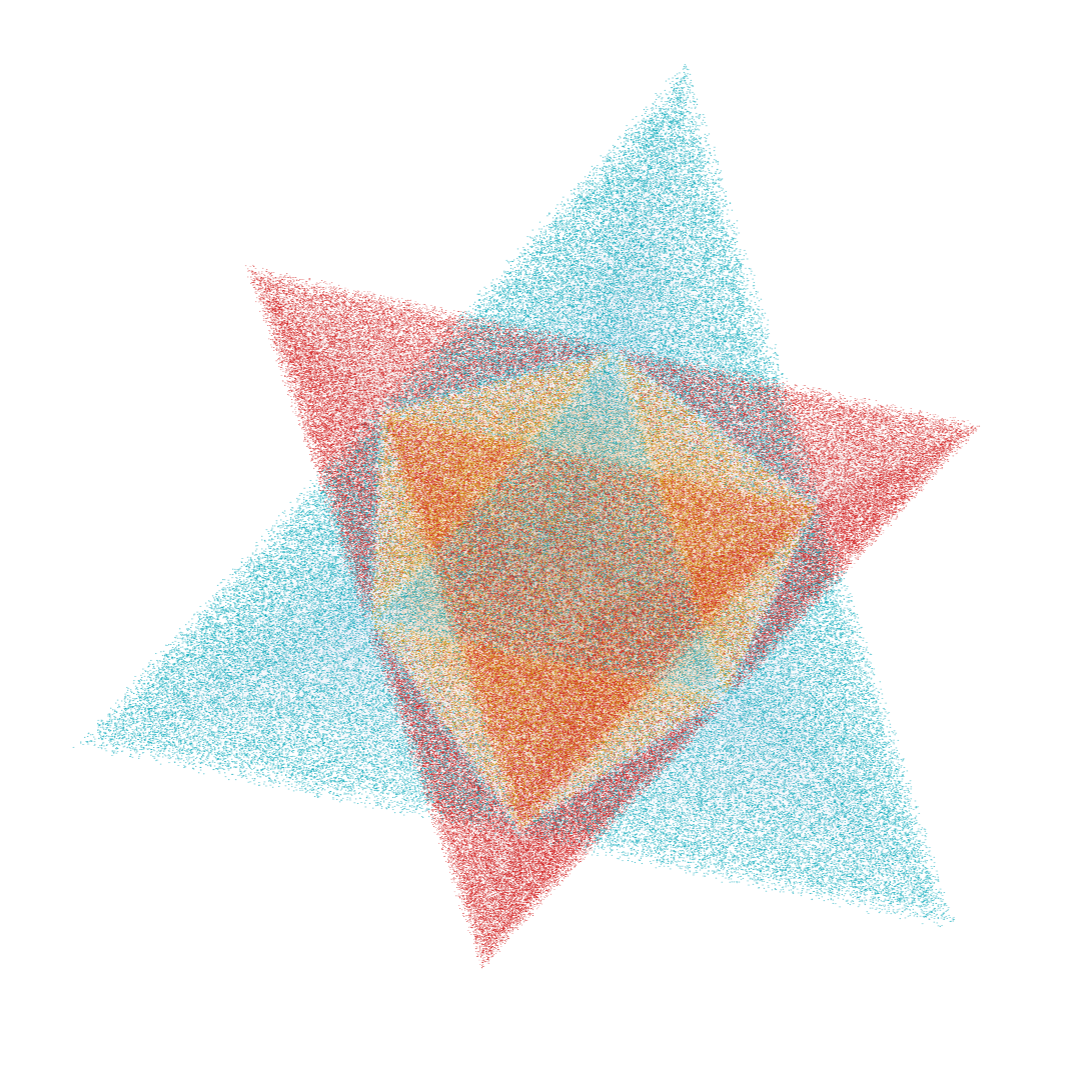
\includegraphics[width=\columnwidth]{fig1_tetrad_frame}
\caption{The coordinate-space geometry of the tetrad frame. Four million points are sampled uniformly in local frame coordinates and classified by the sign combination each point occupies under the four projections $v_i$. The primary tetrahedron (TetA) appears in blue, a second inverted tetrahedron (TetB) in red, and their shared interior, a regular octahedron, in gold. The geometry is analysed in the text. An interactive HTML rendering is provided as supplementary material.}
\label{fig1}
\end{figure}

\section*{Four Planes}

The $(-,+,+,+)$ signature maps null directions in the local frame to
the unit sphere $S^2$. The three identical spacelike entries give the
spatial sector full $SO(3)$ invariance; requiring that a discrete
four-direction set on $S^2$ introduce no net preferred spatial direction
uniquely fixes the regular tetrahedral frame with pairwise inner product
% Lean: reference updated for this note.
$c = -1/3$ (proved in Letter 1's supplementary note on the signature and in
the forced tetrahedral frame proof, whose Lean formalisation this note imports). The four directions,
expressed as linear projections of the local coordinates, are:
\begin{align}
v_1 &= x + y + z, \nonumber \\
v_2 &= x - y - z, \nonumber \\
v_3 &= -x + y - z, \nonumber \\
v_4 &= -x - y + z.
\end{align}

Each projection $v_i$ defines a half-space: the set of all points on one side of the corresponding plane $v_i = \mathrm{const}$. The four planes together close to form a tetrahedron, the unique bounded solid that four planes can enclose. The region where all four projections are simultaneously bounded defines the primary tetrahedral frame, which we label TetA:
\begin{equation}
\textbf{TetA}: \quad \max(v_1,\, v_2,\, v_3,\, v_4) \leq 1.
\end{equation}

Each $v_i$ is the dot product of the position vector with one of the four directions derived above; it measures the displacement of a point along that direction. These projections encode the tetrad's spatial sector in its unique isotropic four-direction basis, playing the role of spatial one-forms projected along the tetrahedral normals rather than the three orthogonal legs. Bounding them as half-space inequalities makes the tetrad's spatial geometry directly computable.

To render this geometry, we sample four million points uniformly in a cube of local frame coordinates, evaluate the four inequalities at each point, and colour each point according to the region it occupies. The geometry emerges from the half-space boundaries alone, without mesh construction or surface fitting. Figure~\ref{fig1} confirms the analytically derived structure described in the following section.

\section*{The Emergent Geometry}

Figure~\ref{fig1} displays the geometry that the four half-space
inequalities produce. The rendering reveals two tetrahedral regions, one
upright (blue) and one inverted (red), overlapping around a compact gold
core. All three regions emerge from the same four planes defined in the
previous section. This section proves which regions must close into finite
solids, why no others can, and identifies the composite solid they form.

Each projection $v_i$ divides coordinate space with a bounding plane. On
one side lies the half-space $\{v_i \leq 1\}$; on the other, its
complement. Replacing $v_i$ with $-v_i$ and applying the same bound gives
the opposite half-space $\{-v_i \leq 1\}$. Since there are four
projections, each offering two choices, there are $2^4 = 16$ ways to
select one half-space per projection. Each selection produces a convex
region, the intersection of four half-spaces. A bounded intersection
closes on itself to form a finite solid; an unbounded one extends to
infinity and has no geometric identity. The natural question is: which of
these sixteen regions are bounded? The answer turns on a single algebraic
identity among the four projections.

In three spatial dimensions, four unit vectors with equal pairwise angles
admit no other configuration than the face normals of a regular
tetrahedron, and face normals of a regular tetrahedron sum to zero. The
four projections therefore satisfy
\begin{equation}
v_1 + v_2 + v_3 + v_4 = 0.
\end{equation}
This identity holds at every point in coordinate space and is the sole
algebraic relation among the four projections. When the inward-pointing
normals of a set of bounding planes sum to zero, the origin sits at their
centroid, strictly inside their convex hull, and the walls close from
every direction; when they do not, a gap opens and the region escapes to
infinity. For TetA, the four inward normals are the derived tetrahedral
directions; they sum to zero, so TetA is bounded. This is unsurprising;
TetA was defined by bounding all four projections.
% Lean: explicit bound.
Explicitly, each $v_i = -\sum_{j\neq i} v_j \geq -3$ on TetA, and the
coordinates are recovered as $x = (v_1+v_2)/2$, $y = (v_1+v_3)/2$,
$z = (v_1+v_4)/2$, so every point of TetA has $|x|,|y|,|z| \leq 3$.

But the same argument applies to the four negated directions: they also sum to
zero, placing the origin at their centroid. A second bounded region
exists, one that was never defined or constructed. This is TetB:
\begin{equation}
\textbf{TetB}: \quad \max(-v_1,\, -v_2,\, -v_3,\, -v_4) \leq 1.
\end{equation}
% Lean: the two regions as tetrahedra.
Writing $\mathbf{n}_a$ for the four directions, so that $v_a = \mathbf{n}_a\cdot\mathbf{p}$,
TetA is the convex hull of the four points $-\mathbf{n}_a$, with barycentric
weights $(1-v_a)/4$, and TetB is the convex hull of the four points
$\mathbf{n}_a$, with weights $(1+v_a)/4$: TetB is the image of TetA under
spatial parity $\mathbf{p}\to-\mathbf{p}$.

No other region can be bounded. Consider any mixed selection, say three
directions that keep their original orientation and one that is flipped. The
linear relation means the flipped direction equals the sum of the other three:
it is a positive combination of them. All four selected normals therefore
point into the same half of space, the origin lies outside their convex
hull, and the region escapes to infinity. The same reasoning applies to
every other mixed selection: flipping any strict subset of the directions breaks
the surrounding property, and the intersection is unbounded.
% Lean: an explicit escape ray for each of the fourteen mixed selections.
Explicitly, let $S$ be the set of directions that keep their orientation,
$1 \leq |S| \leq 3$, and set $\mathbf{d} = -\sum_{b\in S}\mathbf{n}_b$.
Since $\mathbf{n}_a\cdot\mathbf{n}_b = 3$ for $a=b$ and $-1$ otherwise,
$v_c(\mathbf{d}) = |S| - 4 \leq -1$ for $c\in S$ and
$-v_c(\mathbf{d}) = -|S| \leq -1$ for $c\notin S$, so the whole ray
$t\,\mathbf{d}$, $t \geq 0$, lies in the region. Of the
sixteen regions, exactly two close into finite solids: in
Figure~\ref{fig1}, the blue region is TetA and the red region is TetB.
The orientation-reversed tetrahedral sector was not introduced as a
separate frame; it emerges as the unique second bounded region among the
sixteen half-space combinations of a single orthonormal tetrad.

The two tetrahedra interpenetrate: each vertex of TetB passes through a
face of TetA, and each vertex of TetA passes through a face of TetB.
Their intersection is the set of points satisfying $|v_i| \leq 1$ for all
$i$. This region has six vertices, each obtained by setting one
$|v_i| = 1$ and solving for the remaining three under the constraint
$\sum v_i = 0$; all twelve edges are equal in length.
% Lean: the intersection in coordinates.
In coordinates the intersection is $|x|+|y|+|z| \leq 1$, the convex hull of
the six points $\pm\hat{\mathbf{e}}_j$, and each edge has length $\sqrt2$. The intersection is
therefore a regular octahedron, visible as the gold core at the centre of
Figure~\ref{fig1}. The union of the two tetrahedra is a stellated
octahedron, first described by Kepler~\cite{Kepler1619} and known in
modern polyhedral geometry as the stella
octangula~\cite{Cromwell1997}, here derived from the half-space inequalities
of a single orthonormal tetrad.

This interpenetration couples all four faces of each tetrahedron. On each
of the four coupled faces, the opposing vertex carves the face into four
distinct sub-regions: three exposed triangular corners and one central
inverted core. The resulting pattern is the
first level of a Sierpinski subdivision, visible on every face in
Figure~\ref{fig1}. The total number of independent boundary channels
across the four coupled faces follows immediately:
\begin{equation}
4 \;\text{faces} \times 4 \;\text{sub-regions} = 16 \;\text{channels}.
\label{eq:channels}
\end{equation}
Each channel is a distinct connected region of the boundary surface,
separated from its neighbours by the edges where TetA and TetB intersect.
% Lean: the channels as sets.
Precisely, on the face $v_a = 1$ of TetA the core is the part inside TetB,
and the corner $b \neq a$ is the part where $-v_b > 1$; at most one
$-v_b$ can exceed $1$ on the face, so the four pieces are disjoint, they
cover the face, and each is convex and non-empty (the core contains the
face centroid $\mathbf{n}_a/3$, the corner $b$ the vertex $-\mathbf{n}_b$).
Figure~\ref{fig2} illustrates the subdivision for a single face; the
numerical rendering at four million sample points confirms the full count.
Whether deeper levels of the Sierpinski recursion carry geometric
significance is not addressed here.

\begin{figure}[t]
\centering
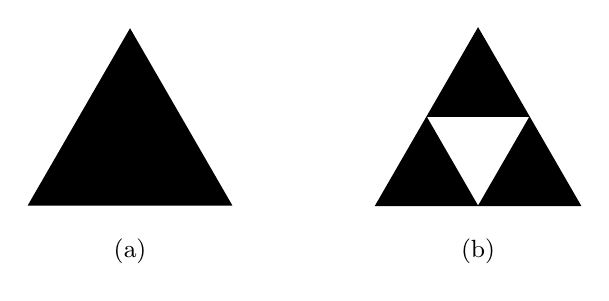
\begin{tikzpicture}[scale=1.3]
  % Panel (a): one solid face of TetA
  \fill[black] (0,0) -- (2,0) -- (1,1.732) -- cycle;
  \node at (1,-0.45) {\small (a)};

  % Panel (b): the same face after TetB's vertex penetrates
  \begin{scope}[xshift=3.4cm]
    \fill[black] (0,0) -- (1,0) -- (0.5,0.866) -- cycle;
    \fill[black] (1,0) -- (2,0) -- (1.5,0.866) -- cycle;
    \fill[black] (0.5,0.866) -- (1.5,0.866) -- (1,1.732) -- cycle;
    \draw[black, line width=0.4pt] (0,0) -- (2,0) -- (1,1.732) -- cycle;
    \node at (1,-0.45) {\small (b)};
  \end{scope}
\end{tikzpicture}
\caption{The face subdivision. (a)~One face of TetA, undivided. (b)~The opposing vertex of TetB penetrates the face, carving it into three exposed corners and one central inverted core. This $3+1$ pattern is the first Sierpinski iteration and repeats on all four faces, producing the $4 \times 4 = 16$ boundary channels of Eq.~(\ref{eq:channels}).}
\label{fig2}
\end{figure}

The three regions visible in Figure~\ref{fig1} are now fully accounted
for. The blue and red tetrahedra are the only bounded regions among the
sixteen half-space combinations; the gold octahedron is their intersection;
and the composite stellated octahedron, with its sixteen boundary channels,
is generated by the half-space inequalities of a single orthonormal tetrad,
with nothing introduced and nothing added.

\section*{Structural Inventory}

Every structural constant of the stellated octahedron that the tetrad produces reduces to two integers: the number of faces per tetrahedron, $K = 4$, and the spatial dimension, $D = 3$. In combinatorial topology, the standard inventory of a polyhedron is its f-vector $(f_0, f_1, f_2)$, recording the number of vertices, edges, and faces. This count is a coordinate-independent combinatorial inventory.

\vspace{6pt}
\noindent
\begin{tabular*}{\columnwidth}{@{\extracolsep{\fill}}lcc@{}}
\hline
Quantity & Expression & Value \\
\hline
Tetrahedra (TetA, TetB) & $2$ & 2 \\
Faces per tetrahedron & $K$ & 4 \\
Vertices (total) & $2^D$ & 8 \\
Edges (total) & $K \times D$ & 12 \\
Faces (total) & $2K$ & 8 \\
Boundary channels & $K^2$ & 16 \\
f-vector sum ($V\!+\!E\!+\!F$) & $K(K\!+\!D)$ & 28 \\
\hline
\end{tabular*}
\vspace{6pt}

\noindent
The f-vector of the stellated octahedron is $(8, 12, 8)$, giving a total element count of $V + E + F = 28$. The alternating sum $V - E + F = 4$ equals twice the Euler characteristic of a sphere, consistent with two simplicially disjoint closed surfaces. Every entry in the table is determined by $K$ and $D$ alone. No additional parameters or geometric inputs are required.

Each tetrahedron individually carries a $3+1$ face decomposition: one face whose normal has uniform sign and three faces with mixed signs, mirroring the $(-,+,+,+)$ Lorentz signature from which the construction began.

% Lean: new section.
\section*{Formal Verification}

Every mathematical statement above is proved in Lean~4 with the Mathlib library,
in \texttt{lean/HalfSpaceTwoBoundedRegions.lean}, and checked by the Lean
kernel. The four directions are imported from the formalisation of the
forced tetrahedral frame, as the columns of its matrix $M$. Boundedness is
Mathlib's \texttt{Bornology.IsBounded}. The file proves: the sole linear
relation (\texttt{proj\_relations}); the classification, a region is bounded
if and only if all four signs agree (\texttt{classification}), so exactly two
of the sixteen are bounded (\texttt{exactly\_two\_bounded}); TetA and TetB as
the tetrahedra with vertices $-\mathbf{n}_a$ and $\mathbf{n}_a$
(\texttt{TetA\_eq\_hull}, \texttt{TetB\_eq\_hull}, \texttt{TetB\_eq\_neg\_TetA});
the interpenetration; the intersection as the regular octahedron
(\texttt{inter\_eq\_octahedron}, \texttt{inter\_eq\_hull\_octVert},
\texttt{octahedron\_regular}); the sixteen channels (\texttt{channels}); the
inventory (\texttt{inventory}); and the $3+1$ sign pattern
(\texttt{three\_plus\_one}). Every theorem depends only on Lean's three
standard axioms. The script \texttt{verify\_half\_space\_two\_bounded\_regions.py}
checks the same claims numerically, by linear programming and convex hulls.

\begin{thebibliography}{9}

\bibitem{Kepler1619}
J.~Kepler,
\textit{Harmonices Mundi} (1619).

\bibitem{Cromwell1997}
P.~R.~Cromwell,
\textit{Polyhedra}
(Cambridge University Press, Cambridge, 1997).

\end{thebibliography}

\end{document}
